\section{Evaluation} \label{section:evaluation}

Lastly, we present an initial evaluation of the 3hop routing protocol in comparison to the RPL routing protocol standard.
Though this is by no means a comprehensive evaluation, we provide evidence that that the 3hop protocol generates less control traffic and results in a better packet reception ratio for realistic application traffic rates.

\subsection{Methodology}

\begin{table}[t]
\centering
\caption{Summary of the results from the four network scenarios using both RPL and 3hop in a single broadcast domain deployment and a multihop deployment}
\label{table:results}
\begin{tabular}{|l|l|l|l|}
\hline
\textbf{Experiment} & \textbf{Reported/Total} & \textbf{PRR min/max} & \textbf{PRR mean/std} \\
\hline
\hline
RPL Single Hop & 10 / 10 & 36\% / 100\% & 82\% / 21\% \\
3hop Single Hop & 10 / 10 & 97\% / 100\% & 98\% / 1\% \\
RPL Multi Hop & 8 / 10 & 48\% / 51\% & 50\% / 1\% \\
3hop Multi Hop & 10 / 10 & 86\% / 100\% & 95\% / 4\% \\
\hline
\end{tabular}
\end{table}


All experiments here were run in an 11 node configuration, with one of the nodes performing as a dedicated border router and root node.
The other 10 nodes generate application traffic at the rate of a single (non-fragmented) packet sent to a server outside the network every 30 seconds.
This packet contains a monotonically increasing counter which is logged at the server and allows us to calculate the packet reception ratio (PRR).
During the experiment, each node also logs the set of transmitted packets, retransmissions and counts of routing protocol control traffic over time; during the reporting phase each node replay this log and relays the data to the coordinating server.

For each routing protocol --- RPL and 3hop --- we execute this scenario for two topologies:
\begin{itemize}
\item Single-hop: all nodes were placed in a 1 sq foot area next to the border router.
In this scenario, \emph{there is no need for a routing protocol}, so the vital metric is how well the routing protocol can ``get out of the way'' of the application traffic.
\item Multi-hop: all nodes were distributed over a \todo{Xm by Xm} lab space with metal desks, cabinets and other obstructions assisting the formation of a multi-hop topology.
In this scenario, the primary metric is the packet delivery ratio (which is assumed to be high in the single-hop case).
\todo{make the diagram}
\end{itemize}

The results of the experiements are summarized in Table~\ref{table:results}.

\subsection{Single-Hop}

\begin{figure}[t]
\centering
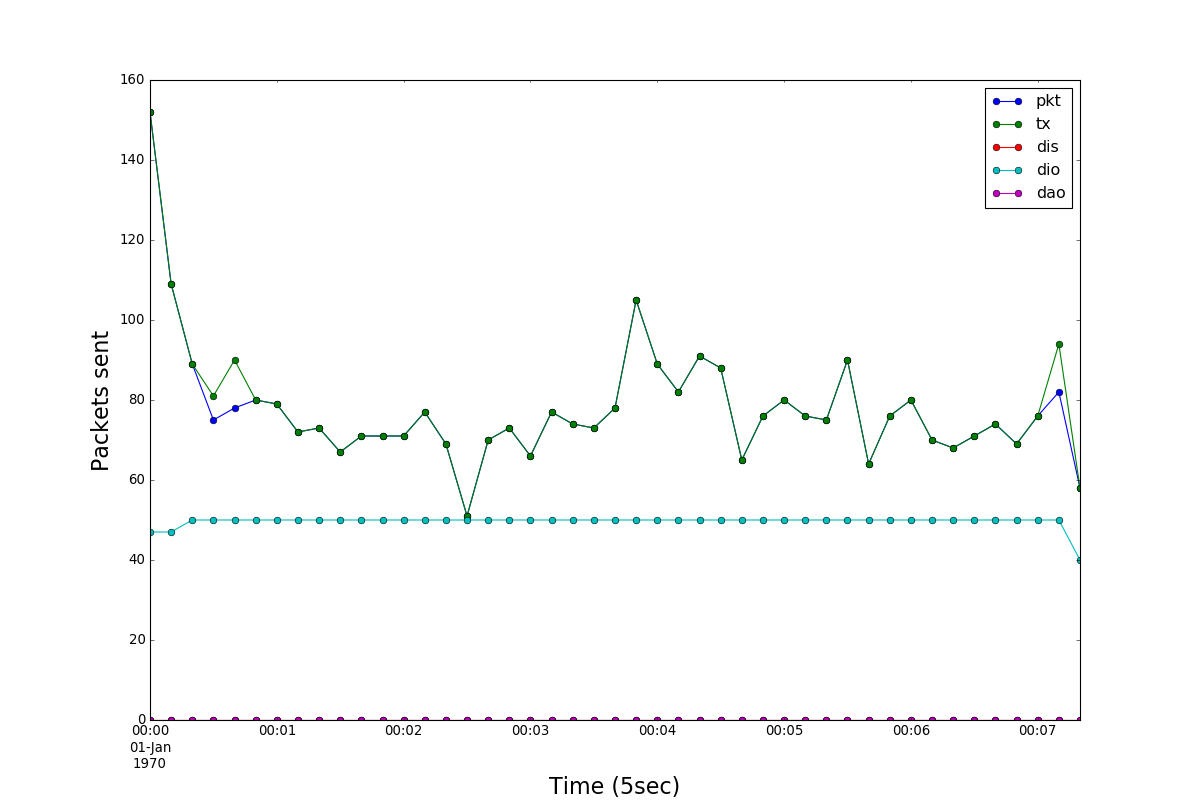
\includegraphics[width=\linewidth]{figs/rpl_single_hop.png}
\caption{Sum of packet types sent over time over all nodes in a RPL topology of a single broadcast domain.}
\label{fig:rpl_single_hop}
\end{figure}

\begin{figure}[t]
\centering
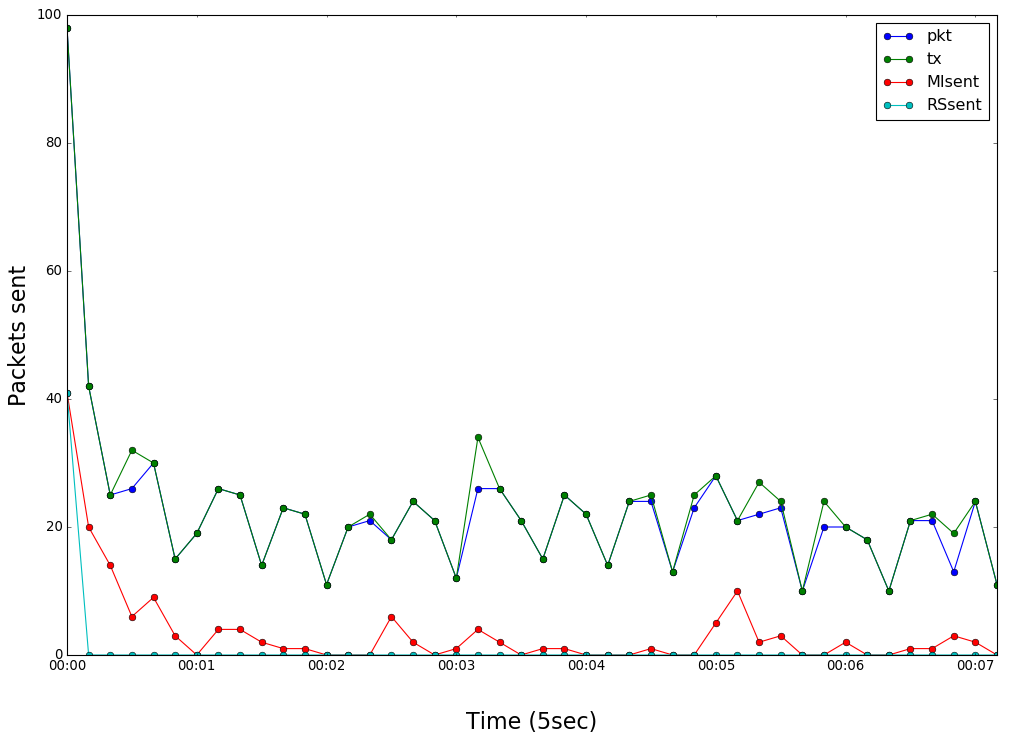
\includegraphics[width=\linewidth]{figs/3hop_single_hop.png}
\caption{Sum of packet types sent over time over all nodes in a 3hop topology of a single broadcast domain.}
\label{fig:3hop_single_hop}
\end{figure}


Here we present the results of the single-hop experiments.
While both protocols achieve similar packet reception ratios, the RPL topology generates roughly twice as many packets because of the constant overhead of DIO advertisement messages.
In contrast, the 3hop protocol generates its equivalent of DIO --- the Router Advertisement messages with the Mesh Info option --- on a Trickle timer, thus reducing the portion of traffic related to maintenance of the topology.

\subsection{Multi-Hop}

\begin{figure}[t]
\centering
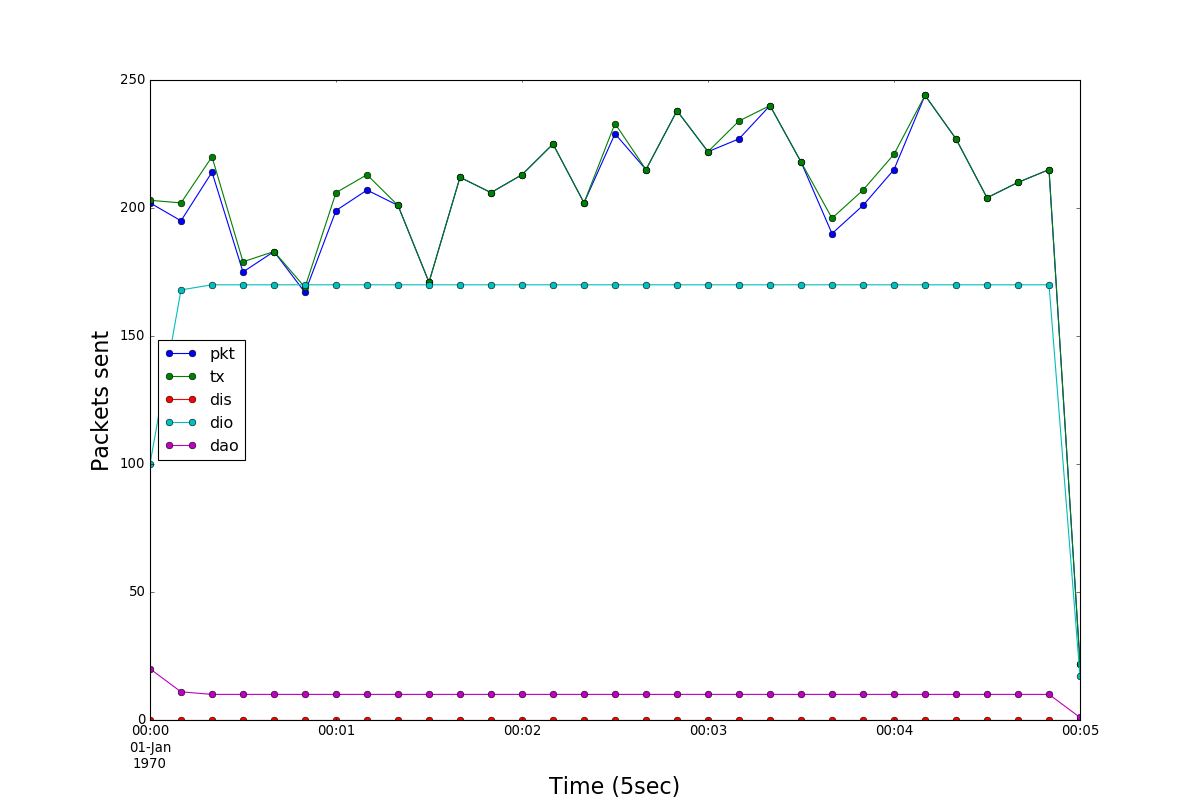
\includegraphics[width=\linewidth]{figs/rpl_multi_hop.png}
\caption{Sum of packet types sent over time over all nodes in a RPL topology of a multi-hop topology.}
\label{fig:rpl_multi_hop}
\end{figure}

\if 0
Want to evaluate the code dissemination part

Describe the methodology:
- what are the aspects of routing protocol we find important, i.e. what are our goals
- given these goals, what do we need to evaluate to demonstrate whether or not we achieved them
- probably want to write the RPL/ipv6 nd discussion first
\fi
